\documentclass[10pt,a4paper,twoside]{article}
% The following LaTeX packages must be installed on your machine: amsmath, authblk, bm, booktabs, caption, dcolumn, fancyhdr, geometry, graphicx, hyperref, latexsym, natbib

%%%%%%%%%%%%%%%%%%%%%%%%%%%%%%%%%PACKAGES
\usepackage{amsfonts, amsmath, amssymb}
\usepackage{bm}
\usepackage{booktabs}
\usepackage{caption}
\usepackage{dcolumn}
\usepackage{fancyhdr}
\usepackage{float}

\usepackage{gensymb}
\usepackage{physics}
\usepackage{upgreek}
\usepackage{xparse}

\usepackage{latexsym}      % needed math symbols
\usepackage{hyperref}
\hypersetup{
 colorlinks=true,
 citecolor=blue,
 linkcolor=blue,
 urlcolor=blue,
 pdfpagemode=UseNone,
 pdfstartview=FitH}
\usepackage{graphicx}      % for importing eps figures
\usepackage[affil-sl]{authblk} 			% found in preprint bundle package, http://ctan.org/pkg/preprint
\usepackage[margin=2.5cm]{geometry} % paper and margin formats as set by SPP
\usepackage{subfig}

%%%%%%%%%%%%%%%%%%%%%%%%%%%%%%%%%

% Please make sure that spp.dat (supplied with this template) is in your working directory or path
\input{spp2025.dat}

%  Editorial staff will uncomment the next line
% \providecommand{\artnum}[0]{XX-XX}
% \renewcommand{\articlenum}[0]{SPP-\the\year-\artnum-}

\begin{document}

%--------------------------------------------------
%  Fill in the paper's title in Sentence case
%  Titles beginning with articles (A, An, The) are discouraged
%--------------------------------------------------
\title{\TitleFont Simulating Spin-Echo MRI Signal Contrast Response to $\vb*{T_R}$–$\vb*{T_E}$ Variations in Tissues with Spatially Varying $\vb*{T_1}$–$\vb*{T_2}$ Maps}


%--------------------------------------------------
% For TWO authors with the same affiliation please use this block
% Or Please use the other author block templates
%--------------------------------------------------
%\author[*\negthickspace]{Author M.~Surname}
%\author[ ]{Bauthor D.~Surname~III\lastauthorsep}
%\affil[ ]{Department of Science, XXX University, Country}
%\affil[*]{\corremail{amsurname@university.edu} }

%--------------------------------------------------
%  For three or more authors with the same affiliation please use this block
%--------------------------------------------------

\author[a,*]{Renato III F. Bolo\authorsep}
\author[a]{Aldrin James R. Garcia\authorsep}
\author[a]{Mariane R. Madlangsakay\authorsep}
\author[a]{Crisleo John II E. Martinito\authorsep}
\author[a]{\\ Katlyn Faye B. Nacague\authorsep}
\author[a]{Herbert B. Domingo\lastauthorsep}
\affil[a]{Department of Physical Sciences and Mathematics, University of the Philippines Manila}
% yung nakaindicate sa affil is \affil[ ]{Department of Science, XXX University, Country}
\affil[*]{\corremail{rfbolo@up.edu.ph} }

%--------------------------------------------------
%  For authors with different affiliations please use the following block
%--------------------------------------------------
% \author[1*]{Author M.~Surname\authorsep}
% \author[2]{Bauthor D.~Surname~Jr.\authorsep}
% \author[1,2]{Coauthor G.~Surname~III\authorsep}
% % !!! Please take note that the last author separation is \lastauthorsep instead of \authorsep
% \author[3]{Dauthor G.~Surname\lastauthorsep}
% \affil[1]{Department of Physics, DD University, Country}
% \affil[2]{Department of Science, XX University, Country}
% \affil[3]{Physics Institute, Country}
% \affil[*]{\corremail{amsurname@university.edu} }
\begin{abstract}
\noindent
%--------------------------------------------------
% Include abstract and keywords here
%--------------------------------------------------
Magnetic Resonance Imaging (MRI) signal contrast fundamentally arises from the interplay between tissue-specific relaxation properties—longitudinal ($T_1$) and transverse ($T_2$) times—and sequence timing parameters such as repetition time ($T_R$) and echo time ($T_E$). While conventional spin-echo simulations often assume homogeneous tissue compartments, biological tissues, especially pathological regions like tumors, exhibit spatially varying relaxation properties. This study presents a simulation framework for analyzing how smooth intra-lesion gradients in $T_1$ and $T_2$ modulate spin-echo MRI signal intensity and contrast. Using steady-state solutions of the Bloch equations, a 2D digital phantom with a radially varying lesion was constructed to model voxel-wise relaxation heterogeneity. Simulations incorporated realistic $T_1$ and $T_2$ ranges for gray matter and lesion tissues, and signal maps were generated under varying $T_R$ and $T_E$ settings. Key results demonstrate how subtle variations in relaxation parameters manifest as non-linear signal patterns, with clear implications for image interpretation and contrast optimization. Signal profiles reveal contrast inversions across acquisition regimes, underscoring the diagnostic trade-offs involved in parameter selection. Quantitative evaluation using lesion-to-background contrast ratio (LBCR) and lesion-to-background signal difference (LBSD), including a novel combined metric, illustrates how spatial heterogeneity alters contrast dynamics beyond what uniform models predict. These findings affirm the need to integrate relaxation heterogeneity into both educational simulations and contrast-optimization protocols. By bridging simplified Bloch models with spatially complex tissue properties, this study advances the understanding of MRI contrast formation and provides a computational toolset for evaluating tissue detectability under spin-echo conditions.

\keywords{relaxation gradients, non-linear signal patterns, spatial heterogeneity, LBCR, LBSD}

\end{abstract}

\maketitle
\thispagestyle{titlestyle}
%--------------------------------------------------
% the main text of your paper begins here
%--------------------------------------------------

\section{Statement of the Problem}\label{sec:intro}
Magnetic Resonance Imaging (MRI) is a non-invasive diagnostic technique widely used in clinical and research settings for its ability to produce detailed anatomical and functional images without ionizing radiation. The contrast in MRI images is fundamentally governed by intrinsic tissue parameters, primarily the longitudinal relaxation time ($T_1$) and the transverse relaxation time ($T_2$) \cite{brown2014}. These parameters reflect how different tissues return to equilibrium after perturbation by radiofrequency (RF) pulses and are critical to understanding signal formation. The time evolution of the net magnetization vector in response to RF excitation and relaxation processes is described by the Bloch equations \cite{bloch1946}.

In particular, spin-echo sequences—common in both clinical and research MRI—yield a steady-state solution to the Bloch equations that relates signal intensity to $T_1$, $T_2$, repetition time ($T_R$), and echo time ($T_E$) \cite{bernstein2004}. This steady-state solution forms the basis for simulating and interpreting MRI contrast. Most introductory and educational simulations rely on simplifying assumptions, including the notion that tissue compartments are homogeneous in their relaxation properties. However, this abstraction oversimplifies the complexity of biological tissues, especially under pathological conditions.

Although $T_1$ and $T_2$ describe intrinsic tissue characteristics, the imaging parameters $T_R$ and $T_E$ play an equally crucial role in shaping the observed signal contrast. The choice of $T_R$ governs the extent of longitudinal recovery between excitations, while $T_E$ determines how much transverse signal decay is captured at readout. Together, these timing parameters modulate sensitivity to different tissue types and heterogeneities. As such, understanding the interaction between $T_1$, $T_2$, $T_R$, and $T_E$ is essential not only for optimizing contrast but also for interpreting variations in signal intensity in regions where relaxation times vary spatially \cite{bernstein2004}.

In reality, tissues often exhibit intra-regional heterogeneity in relaxation parameters due to variations in cellularity, water content, perfusion, necrosis, or other microstructural and physiological processes \cite{tofts2003}. For instance, tumors may contain a mixture of viable cells, necrotic cores, and edematous regions, each with subtly different $T_1$ and $T_2$ values. While these variations may not produce overt visual differences in standard MR images, they influence the local signal response and can affect both qualitative and quantitative interpretations of the image.

This project focuses on understanding how spatial variations in $T_1$ and $T_2$ values within a single tissue region impact the resulting MRI signal, using numerical simulations grounded in the steady-state Bloch model. By going beyond homogeneous-tissue models, the study seeks to explore the degree to which intra-regional relaxation heterogeneity affects signal intensity and image contrast. Such insights are relevant for both medical imaging applications, where accurate tissue characterization is essential, and fundamental physics, where a detailed understanding of signal formation informs the design and interpretation of MR experiments. In particular, the effects of varying acquisition parameters, specifically $T_R$ and $T_E$, are  investigated to determine their role in modulating contrast under relaxation heterogeneity.

\section{General Purpose of the Study}\label{sec:generalobjectives}
The purpose of this study is to examine how spatial variations in $T_1$ and $T_2$ affect spin-echo MRI signal and contrast, using simulations based on the steady-state Bloch model to explore the influence of $T_R$ and $T_E$ on contrast optimization.

\section{Specific Objectives}\label{sec:specificobjectives}
To accomplish this, the study specifically aims to:
\begin{enumerate}
    \item Derive the steady-state spin-echo MRI signal equation from the Bloch equations under relaxation and pulse sequence assumptions appropriate to clinical acquisition;
    \item Construct a 2D digital phantom with spatially varying $T_1$ and $T_2$ maps to simulate signal intensity distributions and generate corresponding contrast metric maps; and
    \item Systematically vary $T_R$ and $T_E$ over clinically relevant ranges and determine parameter combinations that maximize lesion-to-background differentiation.
\end{enumerate}

\section{Review of Related Literature}\label{sec:rrl}

Magnetic Resonance Imaging (MRI) leverages the relaxation properties of nuclear spins---longitudinal ($ T_1 $) and transverse ($ T_2 $)---to generate high-contrast images of soft tissues without ionizing radiation. The time evolution of magnetization under these relaxation processes is governed by the Bloch equations \cite{bloch1946}, forming the theoretical foundation of MRI. In the context of spin-echo sequences, the steady-state signal intensity can be described as
\begin{equation}
S(x, y) = \rho \left[ 1 - e^{-T_R/T_1(x, y)}\right] e^{-T_E/T_2(x, y)},
\label{eq:signal}
\end{equation}
where $ \rho $ is the proton density, and $T_R$ and $T_E$ are the repetition and echo times, respectively \cite{bernstein2004}. This formulation provides a direct quantitative relationship between tissue-specific relaxation parameters and image contrast \cite{brown2014}.

Relaxation times vary significantly between tissue types and are influenced by imaging parameters and magnetic field strength. For example, Stanisz et al.\ \cite{stanisz2005} measured $ T_1 $ values in gray matter at 1.5 T, which is a widely used field strength for modern MRI machines \cite{brown2014}, to be within the range $1124 \pm 50$ ms, and $ T_2 $ values between $95 \pm 8$ ms. Bojorquez et al.\ \cite{bojorquez2017} further demonstrated that acquisition protocols and scanner-specific settings introduce substantial variability, highlighting the importance of reproducibility in clinical interpretation. Moreover, pathologies such as tumors often exhibit altered relaxation profiles due to changes in water content, cellular architecture, or necrosis, as noted in Tofts' review of quantitative MRI in disease states \cite{tofts2003}.

Emerging work has shown that spatial heterogeneity in relaxation parameters can meaningfully affect image contrast. Does et al.\ \cite{does2002} observed multicomponent $ T_1 $ relaxation in rat brain tissue, attributing the behavior to underlying microstructural variations. Xu et al.\ \cite{xu2009} similarly showed that $ T_2 $ variability affects the accuracy of diffusion-weighted imaging, emphasizing the clinical impact of intra-tissue relaxation differences. Despite this, many MRI models assume homogeneity across regions of interest, which may limit their realism in depicting diseased tissues.

Efforts to standardize quantitative MRI across platforms have underscored persistent challenges. A recent multi-center study using the NIST/ISMRM phantom reported inter-scanner variability in $ T_1 $ and $ T_2 $ under 7\%, but confirmed that minor discrepancies can still affect quantitative outcomes \cite{pasini2025}. Furthermore, myocardial studies by Wiesmüller et al.\ \cite{wiesmueller2020} revealed notable intra-segmental $ T_2 $ variation even under consistent imaging conditions, thus underscoring the importance of incorporating spatial gradients in modeling signal formation.

Computational simulations using the Bloch equations offer a tractable framework for exploring these phenomena under controlled conditions. Recent tools such as \texttt{BlochSim.jl} \cite{blochsim} and other open-source packages for MRI signal modeling provide accessible environments for simulating magnetization dynamics, but typically assume spatial uniformity in tissue parameters. As such, simulations incorporating spatially varying $ T_1 $ and $ T_2 $ maps remain underutilized, despite their potential to visualize how subtle tissue gradients manifest as signal heterogeneity.

While spatial heterogeneity in $ T_1 $ and $ T_2 $ presents a crucial dimension in tissue modeling, the interplay between these relaxation parameters and acquisition settings—particularly the repetition time ($T_R$) and echo time ($T_E$)—also fundamentally shapes signal behavior. Optimal selection of $T_R$ and $T_E$ is essential for maximizing lesion conspicuity and diagnostic performance. Hendrick et al.\ \cite{hendrick1984} demonstrated, through Bloch-equation modeling, that CNR in spin-echo MRI is sensitive to interpulse delays, identifying parameter regimes that maximize signal discrimination between tissues. 

More recently, Ragot and Chen \cite{ragot2019} challenged the assumption that $ T_E = T_2 $ yields maximal contrast, showing via physiological-noise modeling that shorter echo times (around 50 ms at 3 T) often outperform nominal $ T_2 $-matching in terms of CNR. Furthermore, the concept of lesion-to-background contrast ratio (LBCR) has gained traction in clinical studies as a robust proxy for lesion detectability, though optimization of $T_R$ and $T_E$ specifically for LBCR in spin-echo imaging remains underexplored. These findings underscore the need to account for both spatially varying tissue properties and acquisition parameter sensitivity when modeling MRI signal formation.

In summary, while theoretical models and standardization phantoms have greatly improved our understanding of MRI contrast, there remains a gap in simulating how smooth spatial variations in relaxation parameters within lesions influence signal intensity under spin-echo conditions. This study addresses that gap by implementing voxel-wise relaxation maps within a 2D phantom, providing insight into the interplay between tissue heterogeneity and MRI signal behavior as a step toward bridging simplified simulations and the complex biological realities of clinical imaging.

\section{Methodology}\label{sec:methods}

\subsection{Overview}

This project simulated the MRI signal produced by a tissue slice with spatially varying relaxation times under a spin-echo pulse sequence. A 2D matrix (phantom) was used to represent a 25-pixel cross-sectional slice, where the background tissue was homogeneous gray matter and a circular lesion was embedded at the center. While the background had fixed longitudinal and transverse relaxation values ($T_1$, $T_2$), the lesion region exhibited radial gradients in both parameters, simulating intra-lesion heterogeneity.

The net magnetization vector $\vb{M}(t)$ evolves according to the Bloch equations:
\begin{align}
\frac{d\vb{M}}{dt} = \gamma \vb{M} \times \vb{B} - 
\begin{bmatrix}
    M_x / T_2 \\
    M_y / T_2 \\
    (M_z - M_0)/ T_1
\end{bmatrix}
\end{align}
where $ \gamma $ is the gyromagnetic ratio, $ \vb{B} $ is the effective magnetic field, and $ M_0 $ is the equilibrium magnetization. For this simulation, we considered the steady-state signal under a spin-echo imaging sequence.

\subsection{Signal Equation (Spin-Echo)}

In a conventional spin-echo (SE) imaging sequence with repeated radiofrequency (RF) excitations, the observable signal intensity at each voxel $(x, y)$ can be modeled. After an initial transient period, the longitudinal magnetization reaches a dynamic equilibrium. If the repetition time ($T_R$) is sufficiently long for the transverse magnetization to decay to zero before the next RF pulse, the system is said to be in a steady-state incoherent (SSI) condition. 

To simplify the derivation of the steady-state spin-echo signal, we made the following common assumptions:
\begin{enumerate}
    \item The derivation is performed in a rotating frame of reference that precesses at the Larmor frequency, which simplifies the precession term in the Bloch equations and makes the effects of RF pulses easier to visualize.
    \item RF pulses ($90^\circ$ and $180^\circ$) are assumed to be instantaneous, meaning they rotate the magnetization without any relaxation occurring during the pulse itself.
    \item The $90^\circ$ pulse rotates $M_z$ to $M_{xy}$, and the $180^\circ$ pulse flips $M_{xy}$ to $-M_{xy}$ and $M_{z}$ to $-M_{z}$.
    \item The steady-state incoherent (SSI) condition is considered, where any residual transverse magnetization from the previous repetition is assumed to have fully decayed before the next excitation pulse. This is generally valid for long $T_R$ values.
    \item The effects of macroscopic motion (flow) and microscopic random motion (diffusion) on the signal are ignored.
    \item A uniform proton density ($\rho$) is assumed throughout the tissue, which is multiplied at the end to represent the available magnetization.
\end{enumerate}

Let the longitudinal magnetization just before the $90^\circ$ excitation pulse be $M_{z,T_R}^-$. The transverse magnetization is assumed to be zero in the steady-state incoherent case. Then, the $90^\circ$ pulse rotates $M_{z,T_R}^-$ into the transverse plane. So, immediately after the pulse:
\begin{align*}
M_{xy}(0) &= M_{z,T_R}^- \\
M_z(0) &= 0
\end{align*}

During this period, the transverse magnetization decays due to $T_2$ relaxation, and the longitudinal magnetization recovers due to $T_1$ relaxation:
\begin{align*}
M_{xy}(t) &= M_{xy}(0) \cdot e^{-t/T_2} \\
&= M_{z,T_R}^- \cdot e^{-t/T_2} \\
M_z(t) &= M_0(1 - e^{-t/T_1}) \quad (\text{since } M_z(0)=0 \text{ and it recovers towards } M_0)
\end{align*}

At $t=T_E/2$:
\begin{align*}
M_{xy}(T_E/2) &= M_{z,T_R}^- \cdot e^{-(T_E/2)/T_2} \\
M_z(T_E/2) &= M_0 \left[ 1 - e^{-(T_E/2)/T_1}\right]
\end{align*}

The $180^\circ$ pulse rephases the transverse magnetization and inverts the longitudinal magnetization.
The phase of $M_{xy}$ is effectively flipped, but its magnitude remains unchanged by the ideal $180^\circ$ pulse for the purpose of the echo formation. The dephasing that occurred is reversed:
\begin{align*}
M_z(T_E/2)^+ = -M_z(T_E/2)^- = -M_0 \left[ 1 - e^{-(T_E/2)/T_1} \right]
\end{align*}

The transverse magnetization now rephases and continues to decay due to $T_2$ relaxation. The longitudinal magnetization continues to recover towards $M_0$. At the echo time ($t=T_E$), the signal is maximum due to rephasing. The transverse magnetization at the echo ($S_{\text{echo}}$) is the remaining magnitude of the transverse magnetization from before the $180^\circ$ pulse, now further decayed for another $T_E/2$ duration:
\begin{align*}
S_{\text{echo}} &= M_{xy}(T_E/2) \cdot e^{-(T_E/2)/T_2} \\
&= \left[ M_{z,T_R}^- \cdot e^{-(T_E/2)/T_2}\right] \cdot e^{-(T_E/2)/T_2} \\
S_{\text{echo}} &= M_{z,T_R}^- \cdot e^{-T_E/T_2}
\end{align*}

The longitudinal magnetization $M_z$ at $t=T_E$ will recover from its inverted state:
\begin{align*}
M_z(T_E) &= M_0 + \left[M_z(T_E/2)^+ - M_0 \right] e^{-(T_E/2)/T_1} \\
M_z(T_E) &= M_0 + \left\{ -M_0 \left[ 1 - e^{-(T_E/2)/T_1}\right] - M_0\right\} e^{-(T_E/2)/T_1} \\
M_z(T_E) &= M_0 + \left[ -M_0 + M_0 e^{-(T_E/2)/T_1} - M_0\right] e^{-(T_E/2)/T_1} \\
M_z(T_E) &= M_0 + \left[ -2M_0 + M_0 e^{-(T_E/2)/T_1}\right] e^{-(T_E/2)/T_1} \\
M_z(T_E) &= M_0 - 2M_0 e^{-(T_E/2)/T_1} + M_0 e^{-T_E/T_1}
\end{align*}

After the echo, the transverse magnetization is assumed to have decayed to zero for SSI. The longitudinal magnetization continues to recover during the remaining time $(T_R-T_E)$:
\begin{align*}
M_{z,T_R}^- = M_0 + \left[M_z(T_E) - M_0\right] e^{-(T_R-T_E)/T_1}
\end{align*}

Substitute $M_z(T_E)$:
\begin{align*}
M_{z,T_R}^- &= M_0 + \left[ M_0 - 2M_0 e^{-(T_E/2)/T_1} + M_0 e^{-T_E/T_1} - M_0\right] e^{-(T_R-T_E)/T_1} \\
M_{z,T_R}^- &= M_0 + \left[ -2M_0 e^{-(T_E/2)/T_1} + M_0 e^{-T_E/T_1}\right] e^{-(T_R-T_E)/T_1} \\
M_{z,T_R}^- &= M_0 - 2M_0 e^{-T_R/T_1 + T_E/2T_1} + M_0 e^{-T_R/T_1}
\end{align*}

This is where the steady-state condition is used. The initial $M_{z,T_R}^-$ must be consistent with the recovery over $T_R$. While the full derivation can be complex, for the steady-state incoherent (SSI) spin-echo, a simpler and more commonly used approach focuses on the recovery of longitudinal magnetization.

Let $M_L(0)$ be the longitudinal magnetization just after the 90$^\circ$ pulse (which is 0). It recovers towards $M_0$ during $T_R$. After a 90$^\circ$ pulse, $M_z$ is zero. It recovers during $T_R$ to $M_0(1-e^{-T_R/T_1})$. This would be the $M_{z,T_R}^-$ for a simple excitation. 

However, in a spin-echo sequence, the signal is generated from the transverse magnetization. The steady-state incoherent condition implies that the relevant longitudinal magnetization for the next excitation pulse is simply $M_0\left[ 1-e^{-T_R/T_1} \right]$, as any transverse magnetization from the previous sequence has fully decayed.
Thus, the initial longitudinal magnetization available for conversion into transverse magnetization by the $90^\circ$ pulse is given by:
\begin{align*}
M_{z,\text{available}} = M_0 \left[ 1-e^{-T_R/T_1} \right]
\end{align*}

This available longitudinal magnetization is then tipped into the transverse plane and experiences $T_2$ decay over the echo time $T_E$. The $180^\circ$ pulse rephases the vector but does not prevent $T_2$ decay. Therefore, the signal intensity ($S$) at the echo time $T_E$ is proportional to the initial proton density ($\rho$) and the product of the recovery of longitudinal magnetization and the decay of transverse magnetization:
\begin{align*}
S = \rho \cdot M_0 \left[ 1-e^{-T_R/T_1} \right] \cdot e^{-T_E/T_2}
\end{align*}

Assuming $M_0$ is proportional to the proton density $\rho$, we can incorporate $\rho$ directly into the signal equation. If we normalize $M_0$ to 1 (or absorb it into $\rho$), the steady-state transverse magnetization, which is directly proportional to the MRI signals, simplifies to:
\begin{align*}
S(x, y) = \rho \left[ 1 - e^{-T_R/T_1(x, y)}\right] e^{-T_E/T_2(x, y)}. \tag{1}
\end{align*}

\subsection{Simulation Platform}

\subsubsection{Phantom Design and Computational Model}
The simulation platform was implemented in Python primarily using \texttt{NumPy} and \texttt{Matplotlib}. The computational model is based on the steady-state spin-echo signal equation derived from the Bloch equations, where the signal intensity \( S(x,y) \) at each voxel is computed using Equation~\eqref{eq:signal}. 

We constructed a \(128 \times 128\) voxel matrix representing a tissue slice, and a circular lesion of radius 25 pixels was placed at the center. Then, the following parameter values were assigned:

\begin{itemize}
    \item \textit{Background (gray matter):} \(T_1 = 920\) ms; \(T_2 = 100\) ms
    \item \textit{Lesion Center (core):} \(T_1 = 1000\) ms; \(T_2 = 90\) ms
    \item \textit{Lesion Edge:} \(T_1 = 1400\) ms; \(T_2 = 130\) ms
\end{itemize}

The relaxation times used in the simulation were selected to represent a hypothetical but biologically plausible tissue model based on published trends in glioma characterization. While these values do not aim to replicate a specific tissue class, they reflect a relaxation gradient commonly observed in gliomas and peritumoral regions. In particular, studies have reported that infiltrated, non-enhancing peritumoral edema can exhibit prolonged \( T_1 \) and \( T_2 \) values compared to the enhancing tumor core, likely due to blood-brain barrier disruption and increased interstitial fluid content \cite{englund1986,blystad2017}. This manifests as higher relaxation times in the lesion edge relative to the core. Moreover, relaxometry has shown that subtle pathophysiological changes---such as lipid/protein accumulation or diffuse infiltration---can induce heterogeneous relaxation patterns not always visible in structural MR images. As such, the chosen values simulate a plausible gradient of biophysical tissue changes and support synthetic evaluation of contrast behavior under controlled conditions.

Relaxation parameter maps for \( T_1 \) and \( T_2 \) were initialized as uniform backgrounds, onto which a circular lesion was superimposed. Within this lesion, both relaxation times were varied radially to mimic continuous tissue heterogeneity. The spatial variation was defined through linear interpolation between specified core and edge values for \( T_1 \) and \( T_2 \), as described by the following:
\begin{align}
    T_1(x, y) = T_{1,\text{core}} + \left( T_{1,\text{edge}} - T_{1,\text{core}} \right) \cdot \frac{r(x, y)}{r_{\max}} \label{eq:relax1} \\
    T_2(x, y) = T_{2,\text{core}} + \left( T_{2,\text{edge}} - T_{2,\text{core}} \right) \cdot \frac{r(x, y)}{r_{\max}} \label{eq:relax2}
\end{align}
where \( r(x, y) \) is the Euclidean distance from the lesion center and \( r_{\max} \) is the lesion radius.

\subsubsection{Visualization and Data Analysis}

Signal maps were generated for varying combinations of repetition time (\( T_R \)) and echo time (\( T_E \)), allowing for exploration of contrast sensitivity across parameter space. For each \( (T_R, T_E) \) pair, the full 2D image was synthesized by element-wise evaluation of the signal model over the relaxation maps.

Multiple layers of post-processing and visualization were employed to evaluate the effects of relaxation heterogeneity and acquisition parameters on MRI signal contrast.

First, 2D colormaps and 3D surface plots were generated to visualize the spatial distribution of \( T_1 \), \( T_2 \), and the simulated signal intensity. A 1D line profile for signal intensity was generated along the central row to assess transitions across the lesion boundary, with smoothing applied via a moving average filter.

To quantify lesion detectability, we define:
\begin{itemize}
    \item \( \mathcal{L} \subset \Omega \): lesion region (within a circular radius \( R \));
    \item \( \mathcal{B} \subset \Omega \): background region (outside a radius \( R + \delta \), where \( \delta \) is a spatial buffer); and
    \item \( |\mathcal{L}| \), \( |\mathcal{B}| \): number of voxels in lesion and background regions.
\end{itemize}

The mean signal values in each region are:
\begin{align}
\bar{S}_L &= \frac{1}{|\mathcal{L}|} \sum_{\bm{r} \in \mathcal{L}} S(\bm{r}), \ \text{and} \notag \\
\bar{S}_B &= \frac{1}{|\mathcal{B}|} \sum_{\bm{r} \in \mathcal{B}} S(\bm{r}). \notag
\end{align}

Now, two contrast metrics were computed:
\begin{itemize}
    \item \textit{Lesion-to-Background Contrast Ratio (LBCR)} defined as the ratio of average signal within the lesion to the average signal in the background:
    \begin{align}
    \mathrm{LBCR}(T_R, T_E) = \frac{\bar{S}_L}{\bar{S}_B} 
    = \frac{\displaystyle \sum_{\bm{r} \in \mathcal{L}} S(\bm{r}) / |\mathcal{L}|}
           {\displaystyle \sum_{\bm{r} \in \mathcal{B}} S(\bm{r}) / |\mathcal{B}|} \label{eq:lbcr}
    \end{align}
    \item \textit{Lesion-to-Background Signal Difference (LBSD)} defined as the absolute difference between these two signal means:
    \begin{align}
    \mathrm{LBSD}(T_R, T_E) = \left| \bar{S}_L - \bar{S}_B \right|
    = \left| \frac{1}{|\mathcal{L}|} \sum_{\bm{r} \in \mathcal{L}} S(\bm{r}) - \frac{1}{|\mathcal{B}|} \sum_{\bm{r} \in \mathcal{B}} S(\bm{r}) \right| \label{eq:lbsd}
    \end{align}
\end{itemize}

A systematic grid of \( T_R \) and \( T_E \) values was used to compute LBCR and LBSD matrices via Equation~\eqref{eq:lbcr} and Equation~\eqref{eq:lbsd}, enabling contrast analysis over the parameter space. These matrices were visualized as heatmaps to highlight trends and optima. A normalized, weighted combination of LBCR and LBSD was also introduced to balance relative and absolute contrast effects, providing a single composite metric for optimization. Specifically, to balance the strengths of both metrics, a combined contrast metric, $\eta$, was defined as
\begin{align}
    \eta = 0.35 \cdot \text{LBCR}_\text{norm} + 0.65 \cdot \text{LBSD}_\text{norm}. \label{eq:combinedmetric}
\end{align}

The LBSD weight of 0.65 was chosen because absolute signal differences are critical for distinguishing subtle variations within the lesion’s radial relaxation gradients, particularly in clinical settings where lesion boundaries must be clearly delineated \cite{does2002}. The LBCR weight of 0.35 ensures that relative contrast, which aids visual interpretation, remains a contributing factor. 

Finally, to achieve sub-grid precision in optimal  \( (T_R, T_E) \) selection, bilinear interpolation was performed using \texttt{RegularGridInterpolator} over a 25×25 fine grid of linearly spaced $T_R$ and $T_E$ values. The resulting contrast map, derived from combined LBCR and LBSD scores in Equation~\eqref{eq:combinedmetric}, was visualized via filled contour plots (\texttt{contourf}) with 50 levels. The global maximum was highlighted with a red marker to indicate the optimal parameter pair.

\subsubsection{Code Availability}
The complete source code used for phantom generation, spin-echo simulation, and LBCR/LBSD analysis is available at: \url{https://github.com/rntfbliii/ap191-ipmri-project-bloch-mri}. This repository includes the full Python script, input parameters, and output data used in all figures and analysis presented in this paper.



\section{Results and Discussion}\label{sec:rnd}

This section presents the results of the Bloch equation-based simulation framework, evaluating how spatially heterogeneous $ T_1 $ and $ T_2 $ distributions affect spin-echo signal intensity and contrast. Through multi-scale visualization and LBCR-LBSD-based quantification, we investigated how varying acquisition parameters ($T_R$, $T_E$) influence simulated MRI contrast in the presence of tissue heterogeneity, in line with the objectives of visualizing voxel-level signal behaviors and optimizing contrast metrics.

\subsection{Visualization of Relaxation Parameter Maps}

To simulate the impact of intra-lesional heterogeneity, 2D spatial maps of $ T_1 $ and $ T_2 $ values were generated based on plausible gray and white matter ranges \cite{stanisz2005, bojorquez2017}. Figure~\ref{fig:t1t2maps} shows both the 2D projections and their 3D surface representations. The gradual spatial variations in both $ T_1 $ and $ T_2 $ mimic biological tissues where microstructural differences give rise to smooth relaxation gradients, consistent with findings by Does et al.\ \cite{does2002} and Xu et al.\ \cite{xu2009}.

\begin{figure}[htbp!]
\centering
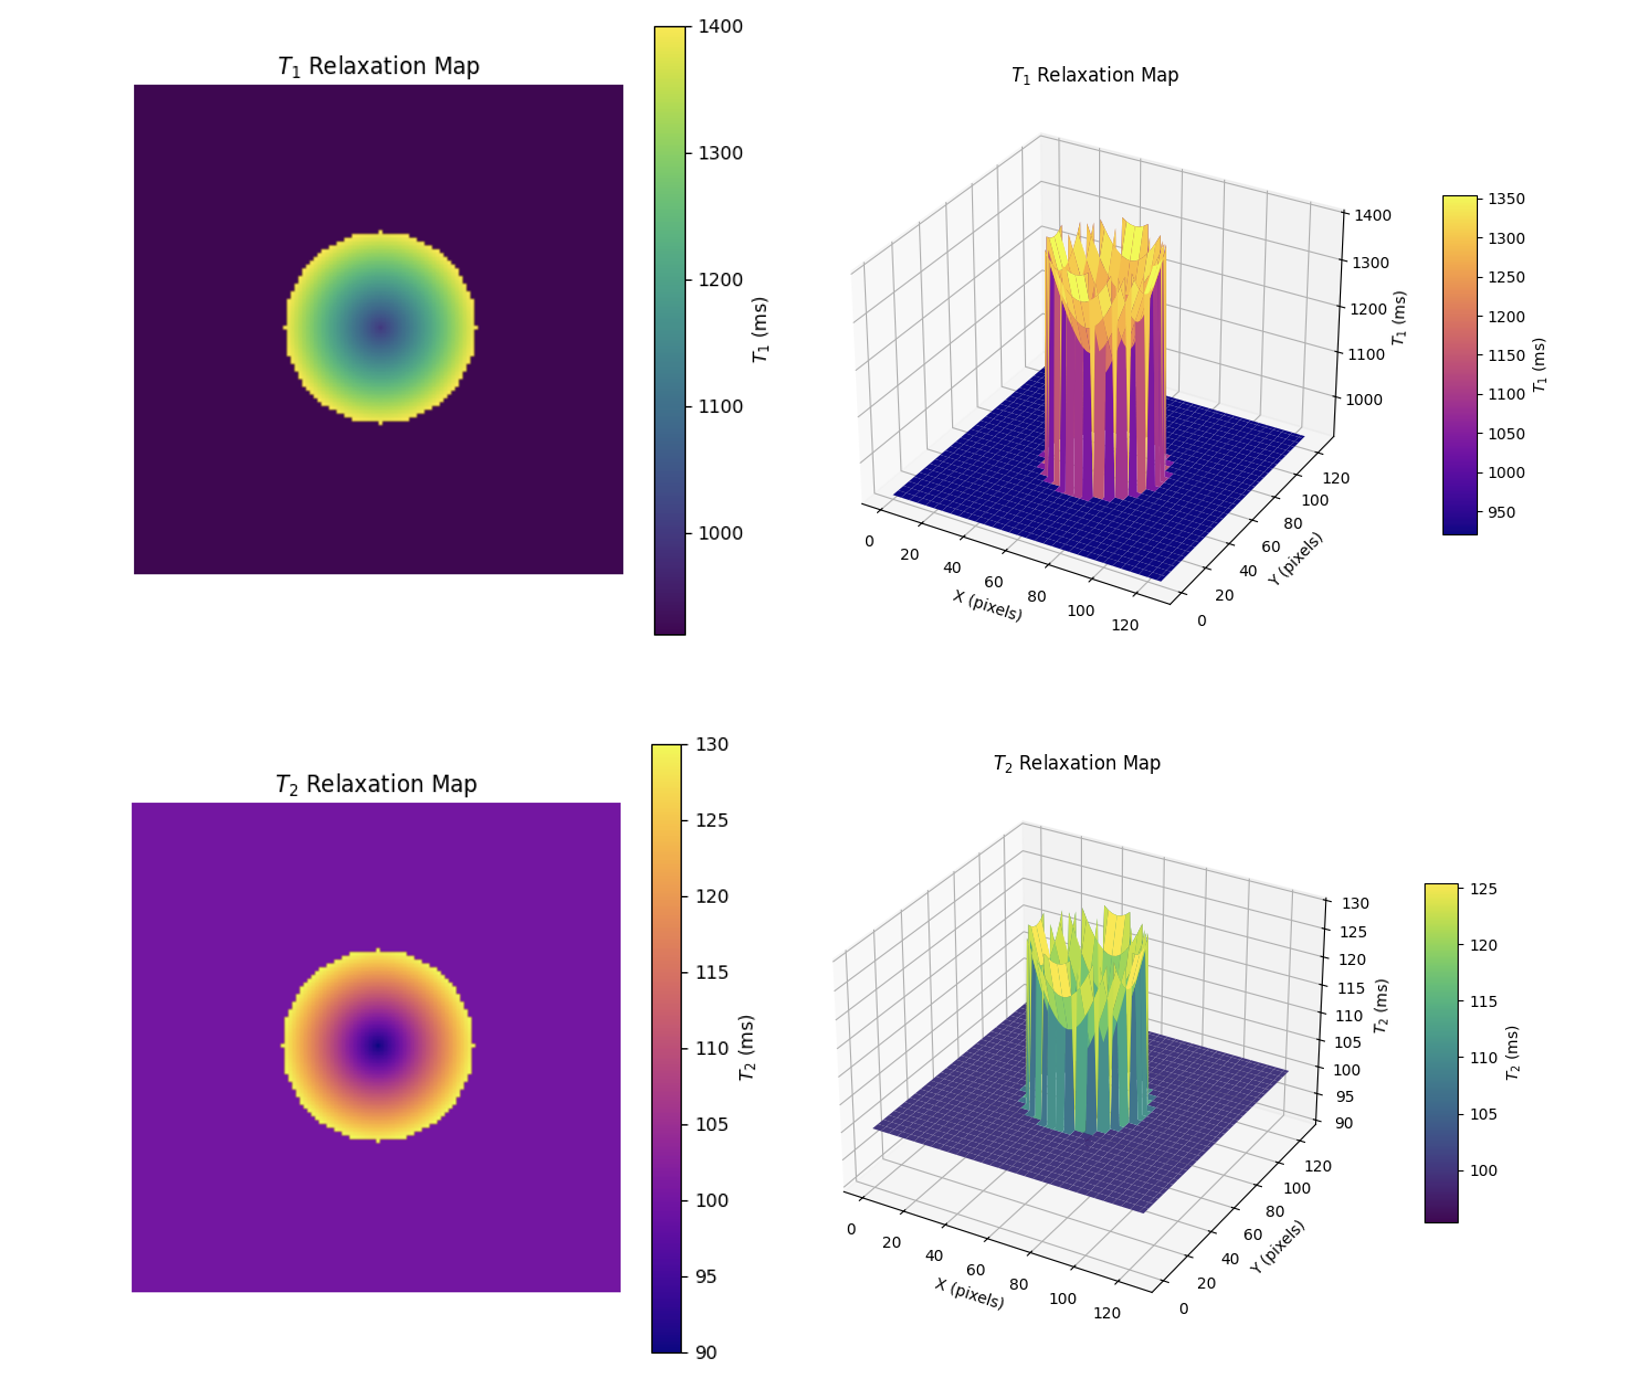
\includegraphics[width=0.7\textwidth]{figures/t1t2maps.png}
\caption{Simulated 2D and 3D spatial distributions of $T_1$ and $T_2$ relaxation times across a heterogeneous lesion phantom. Gradients reflect plausible intra-lesional variation consistent with gray–white matter properties and microstructural tissue differences.}
\label{fig:t1t2maps}
\end{figure}


\subsection{Spin-Echo Signal Map and Line Profile Analysis}

Using Equation~\eqref{eq:signal}, signal intensity was computed voxel-wise for fixed $ T_R = 2000 $ ms and $ T_E = 100 $ ms. The resulting signal map (Figure~\ref{fig:signalmap}) reflects the interplay between proton density-weighted modulation and spatially varying relaxation times. Bright regions correspond to shorter $ T_1 $ and longer $ T_2 $, validating expectations from theoretical contrast behavior \cite{bernstein2004, brown2014}.

To further illustrate spatial variation, a 1D horizontal signal profile was extracted across a representative slice (Figure~\ref{fig:lineprofile}). The gradual decline and curvature of intensity across space highlight how even smoothly varying $ T_1 $ and $ T_2 $ values introduce complex signal patterns, reinforcing the need for spatially resolved models rather than homogenous assumptions.

\begin{figure}[htbp!]
\centering
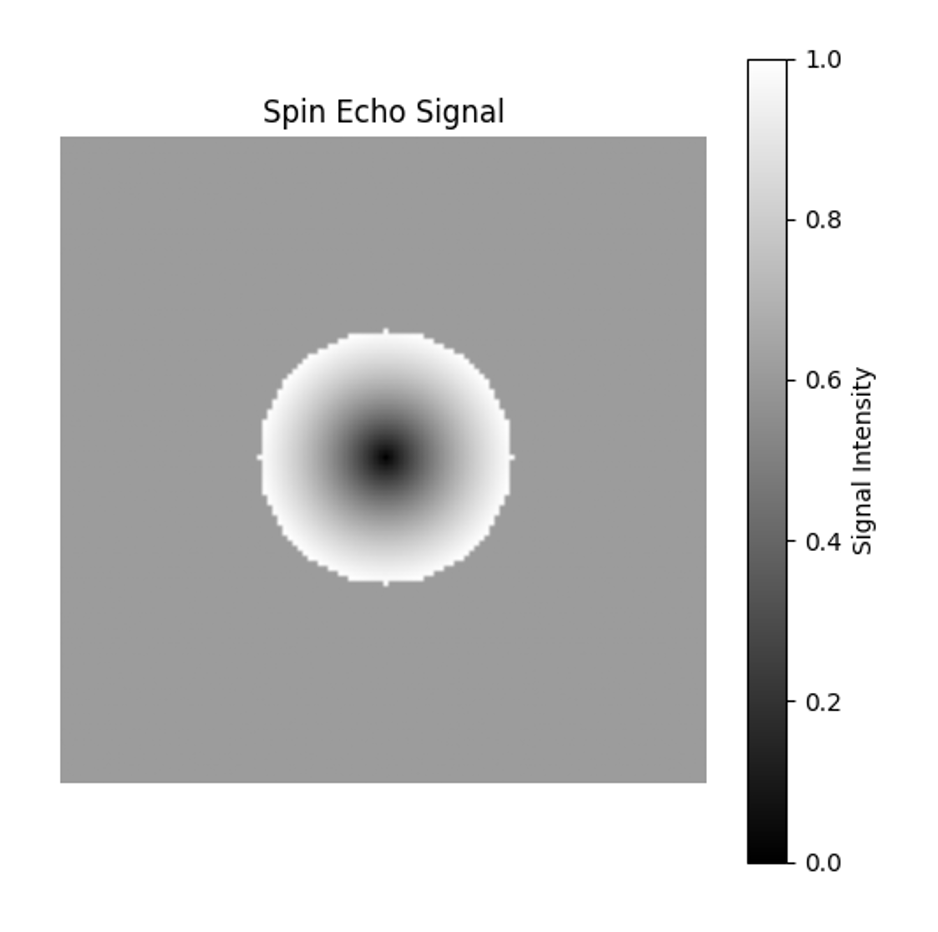
\includegraphics[width=0.4\textwidth]{figures/signalintensitymap.png}
\caption{Voxel-wise spin-echo signal intensity map at $T_R = 2000$ ms and $T_E = 100$ ms, showing spatial contrast shaped by local variations in $T_1$ and $T_2$. Brighter areas reflect favorable relaxation combinations for signal preservation.}
\label{fig:signalmap}
\end{figure}

\begin{figure}[htbp!]
\centering
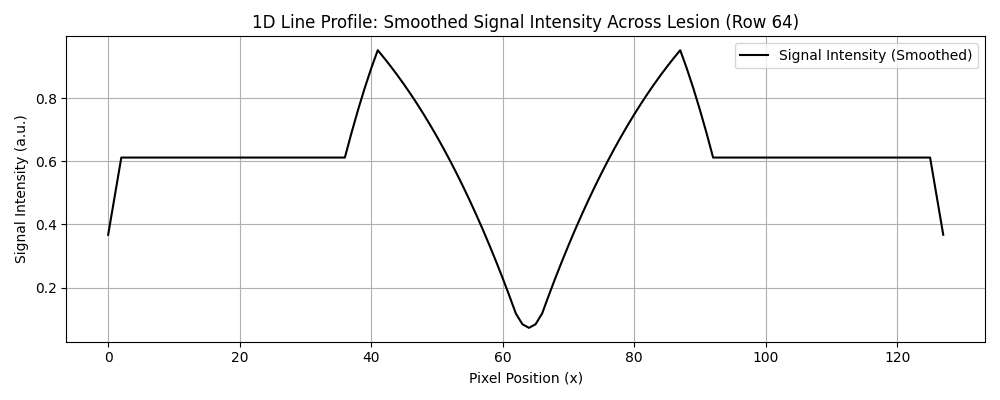
\includegraphics[width=0.8\textwidth]{figures/1Dlineprofilesignal.png}
\caption{1D signal intensity profile extracted along a horizontal slice, illustrating spatial modulation from gradual $T_1$ and $T_2$ changes. Nonlinear trends reflect the cumulative effects of relaxation heterogeneity.}
\label{fig:lineprofile}
\end{figure}

\subsection{Intensity Inversion Across Varying $\vb*{T_R}$ and $\vb*{T_E}$}

To evaluate classical contrast inversion behavior, signal intensities were compared between two representative pulse sequences: one with long repetition and echo times (\( T_R = 2000 \, \mathrm{ms},\ T_E = 100 \, \mathrm{ms} \)) and another with short timing parameters (\( T_R = 800 \, \mathrm{ms},\ T_E = 30 \, \mathrm{ms} \)). As shown in Figure~\ref{fig:inversion}, the relative intensity between the lesion edge and core inverts between the two regimes. This behavior reflects theoretical contrast mechanisms: longer \( T_R \) reduces T1-weighting and favors T2 contrast, enhancing signals from tissues with long \( T_2 \); conversely, shorter \( T_E \) reduces T2 decay and enhances T1-weighted differences. The observed inversion thus exemplifies the tradeoff between T1 and T2 sensitivity, consistent with analytical models and prior literature \cite{brown2014}.

\begin{figure}[htbp!]
\centering
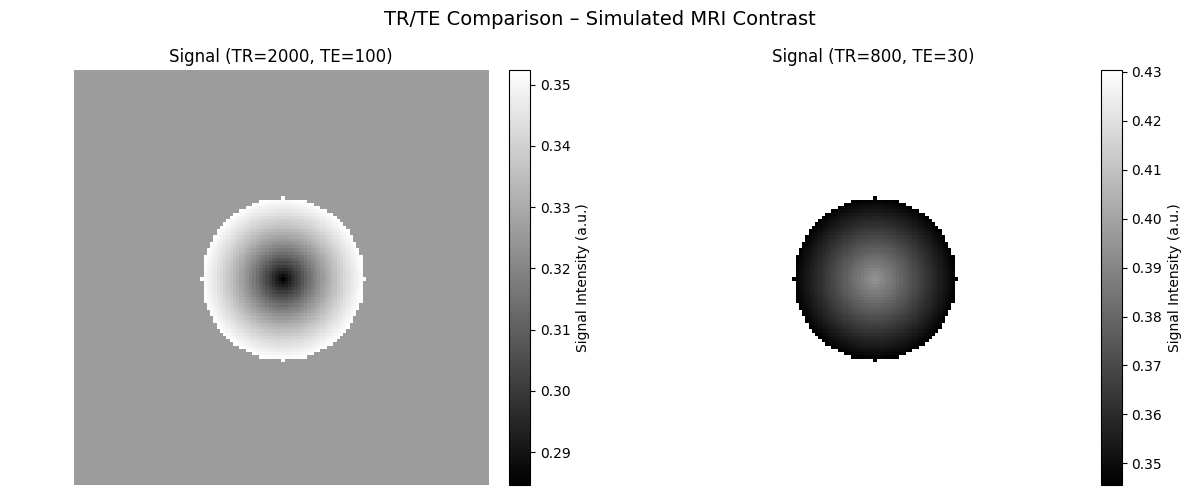
\includegraphics[width=0.8\textwidth]{figures/trtecomparisonforcontrast.png}
\caption{Contrast inversion behavior between (left) long \( T_R = 2000 \ \mathrm{ms},\ T_E = 100 \ \mathrm{ms} \) and (right) short \( T_R = 800 \ \mathrm{ms},\ T_E = 30 \ \mathrm{ms} \). The lesion core and edge exhibit inverted relative signal intensity between these regimes due to shifting $T_1$/$T_2$ contrast mechanisms.}
\label{fig:inversion}
\end{figure}

\subsection{Quantitative Contrast Evaluation Using LBCR and LBSD}

To evaluate the impact of spatially varying \( T_1 \) and \( T_2 \) relaxation times on MRI signal contrast, a 5×5 grid of spin-echo images was generated using combinations of repetition times \( T_R \in \{100, 500, 1000, 1500, 2000\} \) ms and echo times \( T_E \in \{10, 30, 60, 90, 120\} \) ms, as shown in Figure~\ref{fig:grid}. These values were selected to span a range of clinically relevant parameters, enabling a comprehensive assessment of contrast behavior in a simulated 2D tissue phantom with a heterogeneous lesion. The phantom, designed with a circular lesion (radius 25 pixels) embedded in homogeneous gray matter, incorporated radial gradients in relaxation times: \( T_1 \) from 1000 ms (lesion core) to 1400 ms (lesion edge) and \( T_2 \) from 90 ms (core) to 130 ms (edge), with gray matter fixed at \( T_1 = 920 \) ms and \( T_2 = 100 \) ms \cite{stanisz2005, bojorquez2017}.

For each \( T_R \)-\( T_E \) combination, two metrics were computed: the Lesion-to-Background Contrast Ratio (LBCR) via Equation~\eqref{eq:lbcr} and the Lesion-to-Background Signal Difference (LBSD) via Equation~\eqref{eq:lbsd}. Because LBCR can overemphasize contrast at low signal levels, and LBSD can underrepresent relative differences in high-signal regimes, combining both metrics allows for a more robust optimization framework that balances visual contrast and quantitative separability. These metrics build on prior work emphasizing objective contrast evaluation over subjective visual assessment \cite{dewilde1997, mustafa2021}.

\begin{figure}[htbp!]
\centering
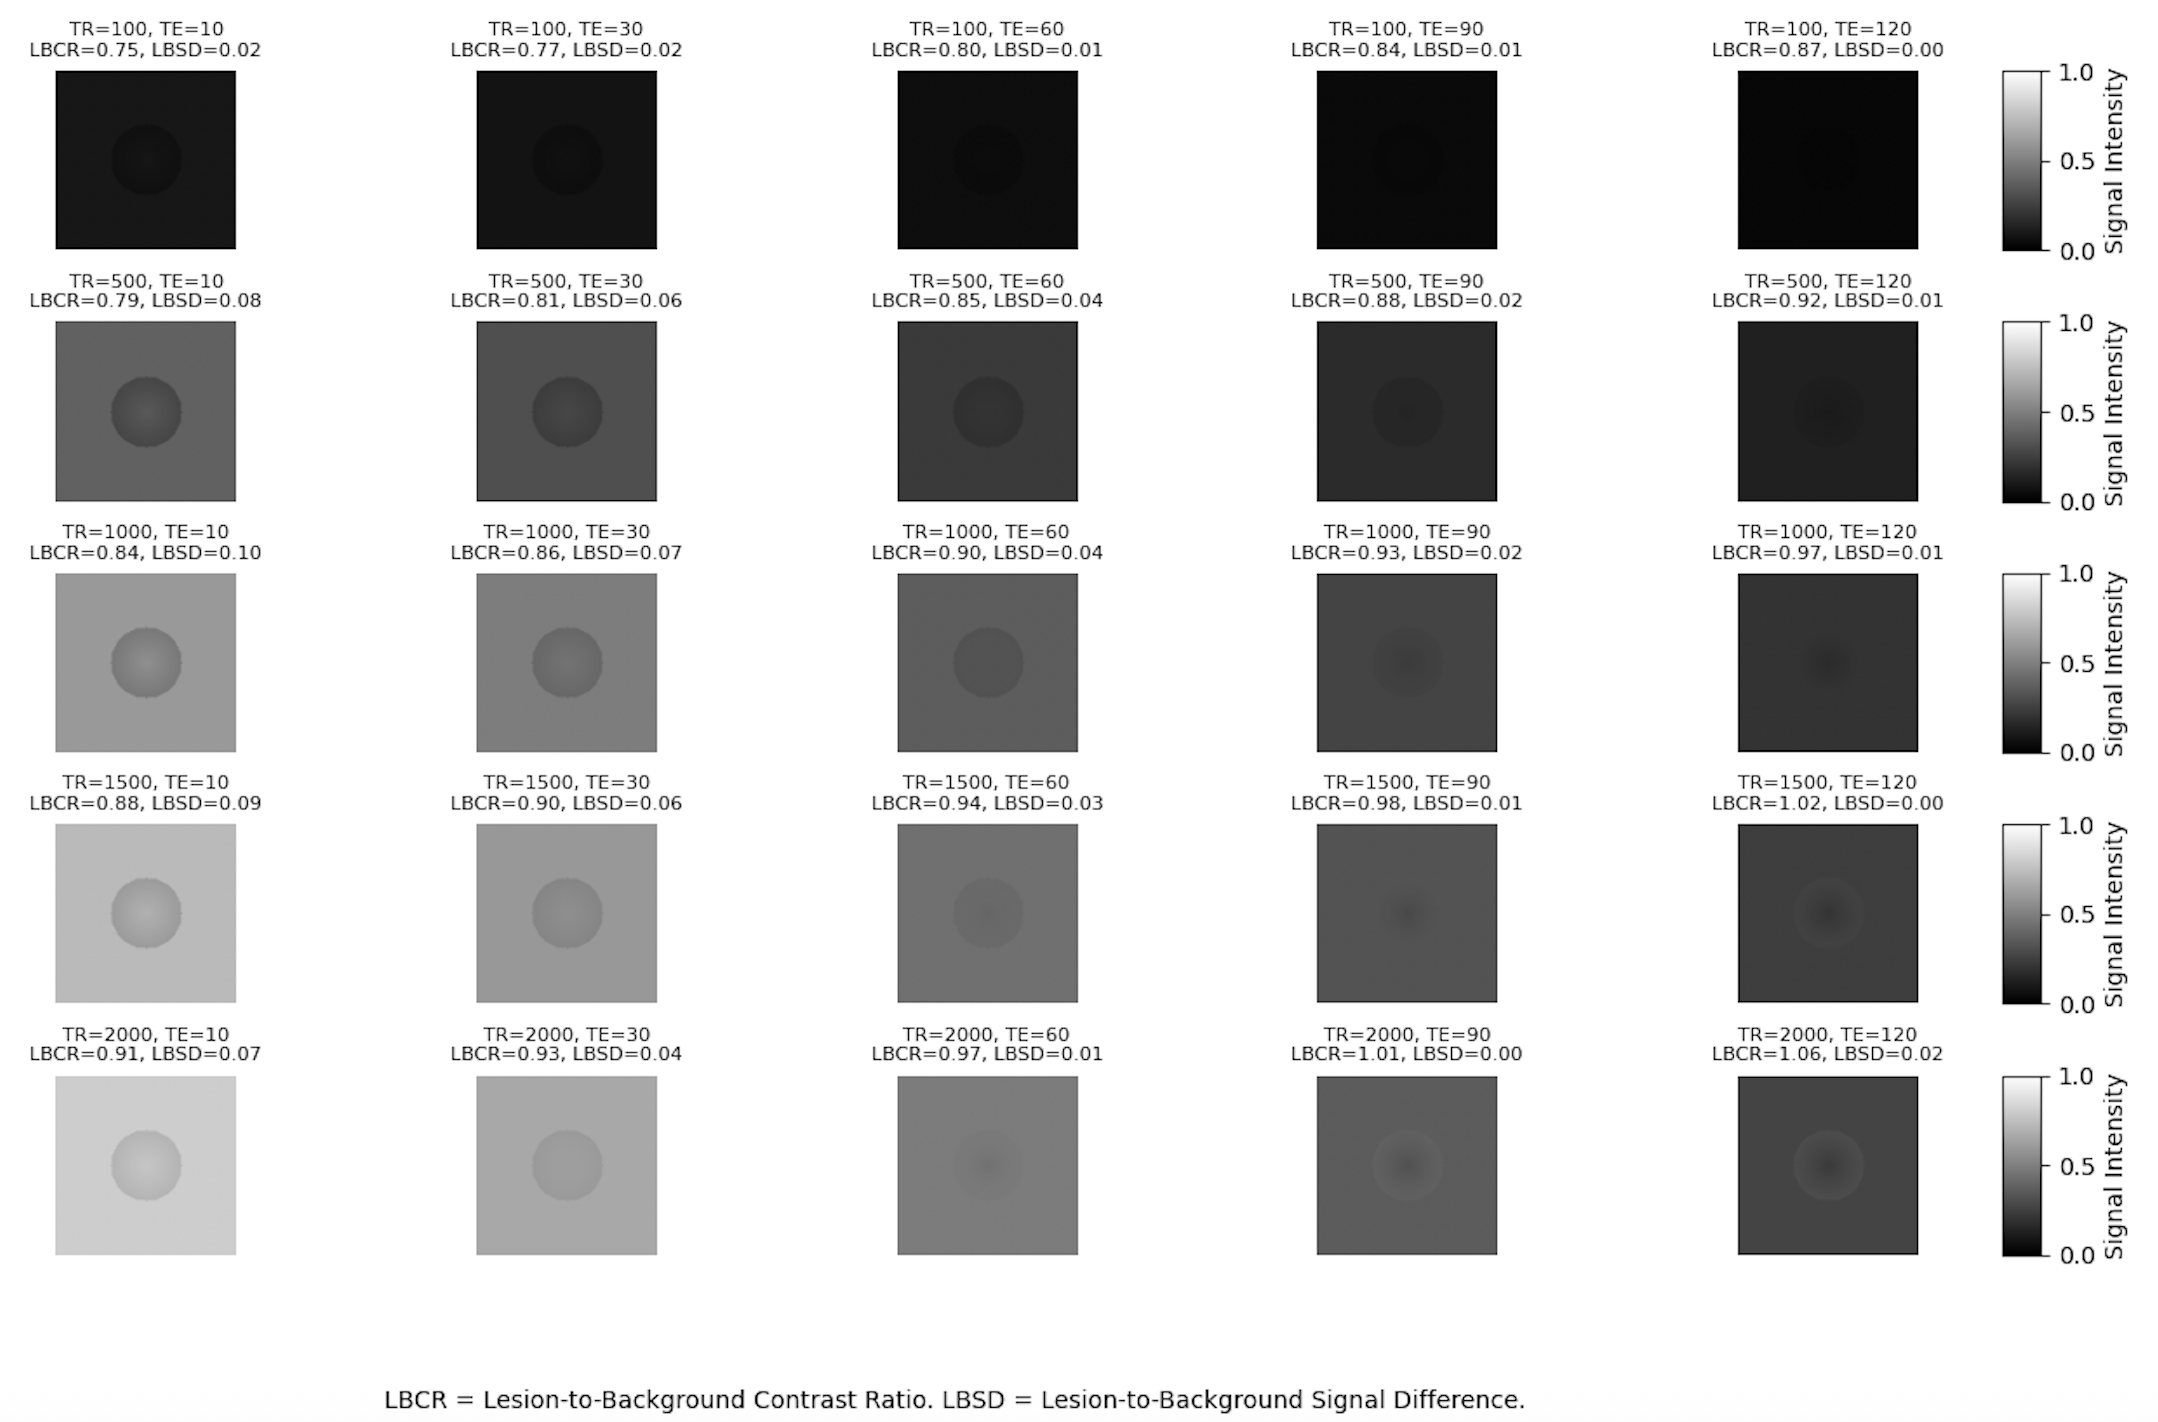
\includegraphics[width=\textwidth]{figures/lbcrlbsdmatrix.png}
\caption{Grid of simulated spin-echo images across combinations of \( T_R \) and \( T_E \), illustrating signal contrast variations in a heterogeneous lesion. Each tile is annotated with LBCR and LBSD values to quantify relative and absolute lesion-background separability.}
\label{fig:grid}
\end{figure}

Analysis of the simulated image grid revealed distinct, non-monotonic contrast behaviors resulting from the interplay between spin-echo timing parameters—repetition time (\( T_R \)) and echo time (\( T_E \))—and spatial heterogeneity in tissue relaxation. The highest LBCR, with a value of 1.06, was observed at \( T_R = 2000 \) ms and \( T_E = 120 \) ms. This configuration allows for substantial longitudinal relaxation recovery in both lesion and background while also maximizing \( T_2 \)-related signal decay, thereby enhancing relative contrast. Conversely, the highest LBSD, reaching 0.10, was found at \( T_R = 1000 \) ms and \( T_E = 10 \) ms, where short echo times preserve absolute signal magnitude differences before substantial transverse decay, and intermediate \( T_R \) values maintain dynamic range across tissues with divergent \( T_1 \) values.

To evaluate combined contrast efficacy, we introduced a hybrid metric composed of a weighted sum of LBCR (35\%) and LBSD (65\%) shown in Equation~\eqref{eq:combinedmetric}. This combined contrast score peaked at the same \( T_R = 1000 \) ms and \( T_E = 10 \) ms configuration, as shown in Figure~\ref{fig:lbcrsurface}. The weighting scheme was selected to prioritize LBSD’s sensitivity to signal intensity separation—critical in detecting subtle intra-lesional variations—while retaining LBCR’s perceptual salience for visual contrast assessment. This approach aligns with the clinical imperative to optimize both detectability and discriminability, particularly in tissues exhibiting radial gradations. Prior studies on contrast optimization and tissue heterogeneity similarly support the necessity of balancing absolute and relative contrast metrics \cite{tofts2003, does2002, xu2009}.

In Figure~\ref{fig:grid}, different signal intensity maps were generated using Equation~\eqref{eq:signal} to simulate varying $T_R$ (100--2000 ms) and $T_E$ (10--120 ms) values. In the figure, darker regions indicate a lower signal intensity while the brighter regions indicate a high signal intensity. The following analysis highlights key \( T_R \)-\( T_E \) combinations to elucidate their impact on contrast:
\begin{itemize}
    \item $T_R=100$ ms and $T_E=10$ ms
    
Short $T_R$ and $T_E$ values typically result to $T_1$-weighted images. However, the image produced at these values appeared to be a low-contrast and low-signal image due to the excessively short $T_R$ value. At $T_R=100$ ms, most lesion components have not yet experienced full $T_1$ recovery, resulting to a lack of contrast in $T_1$ values. This image has produced the lowest LBCR value of 0.75 and a low LBSD value 0.02, denoting a poor lesion-to-background contrast distinction and low signal difference, which is consistent with its observed poor visual visibility and difference between the lesion and background.
    
    \item $T_R=500$ ms and $T_E=10$ ms 

The short $T_R$ and $T_E$ values emphasized $T_1$ contrast while minimizing $T_2$ effects, producing a $T_1-$weighted image with limited longitudinal recovery, reducing dynamic range. The image shows a bright lesion core due to its shorter $T_1$ relaxation, while the lesion periphery remains darker. The configuration yielded an LBCR value of $0.79$, indicating poor lesion-to-background separation despite some visual distinction in the lesion's core, consistent with limited $T_2$ contribution and incomplete longitudinal recovery at the $T_R$.

    \item  $T_R=1000$ ms and $T_E=10$ ms
    
The long but intermediate $T_R$ and short $T_E$ produced an image that balances $T_1$ and $T_2$ effects, yielding a mixed contrast image. The lesion exhibits both internal signal variation and clear differentiation from surrounding tissue. This supports the finding that the combined metric peaked at this point, as seen in the combined LBCR and LBSD heatmap. It produced an LBCR value of $0.84$ and the highest LBSD value of $0.10$. Although the LBCR is not the highest, the significantly high LBSD and overall visual interpretability made this the most effective combination for simultaneously capturing lesion heterogeneity and ensuring adequate lesion-background contrast.

    \item  $T_R=2000$ ms and  $T_E=10$ ms

The long $T_R$ and short $T_E$ values minimize both the $T_1$ and $T_2$ contrast, producing a proton density-weighted image. In this image, the lesion core appeared to be brighter, indicating a high proton density in this area. On the other hand, the lesion edge appeared to be darker with respect to the lesion core, indicating a lower proton density in comparison to its core. This proton density-weighted image has yielded an LBCR value of 0.91, indicating a good lesion-background contrast for viewing proton density differences. However, this image has obtained a lower LBSD value, 0.07, compared to the previous combination yielding 0.10, indicating decreased distinguishability.

    \item $T_R = 1500$ ms and $T_E = 90$ ms

This configuration, with a long \( T_R \) and moderately long \( T_E \), favors \( T_2 \)-weighted contrast. The extended \( T_R \) allows for near-complete longitudinal magnetization recovery, while the long \( T_E \) permits substantial transverse relaxation differences to manifest. In the resulting image, the lesion core appeared relatively darker due to its shorter \( T_2 \), while the peripheral regions appeared brighter, consistent with longer \( T_2 \) values. This spatial heterogeneity yielded an LBCR of 0.98, indicating strong relative contrast. However, the LBSD value was only 0.01, signifying that the absolute signal difference between lesion and background was minimal. As a consequence, despite good relative contrast, the lesion may remain visually ambiguous due to uniformly low signal intensities, which limits the ability to resolve fine structural boundaries in practice.


    \item $T_R = 100$ ms and $T_E = 120$ ms

This combination of a very short \( T_R \) and a long \( T_E \) suppressed signal intensity across all tissues, yielding poor overall contrast. Limited \( T_1 \) recovery and complete \( T_2 \) decay resulted in low signal levels, despite an LBCR of 0.87. However, the LBSD dropped to 0.00, indicating that lesion and background signals were virtually indistinguishable. Thus, the image is diagnostically ineffective despite a seemingly high contrast ratio.


    \item $T_R = 2000$ ms and $T_E = 120$ ms

This configuration, with both a long \( T_R \) and long \( T_E \), accentuates \( T_2 \)-weighted contrast while minimizing \( T_1 \) contributions. The resulting image demonstrates a visibly darker lesion core due to its shorter \( T_2 \) relaxation time, whereas the lesion edges appear brighter, reflecting longer \( T_2 \) values. This spatial variation is characteristic of \( T_2 \)-dominant weighting. The image yielded the highest LBCR value of 1.06, indicating a favorable relative contrast between the lesion and background. However, the LBSD value remained low at 0.02, suggesting that the absolute signal difference is minimal. Despite the strong contrast ratio, the overall signal magnitude in both regions remains low, limiting practical distinguishability. This illustrates that a high LBCR does not necessarily imply strong visual contrast, especially when signal levels are uniformly suppressed.

    


%    \item \textit{Short $T_R$ (500 ms) and Short $T_E$ (10ms) Values}. The short $T_R$ and $T_E$ values minimizes $T_2$ contrast, producing a $T_1$-weighted image. In this image, the lesion core appeared to be brighter due to a shorter $T_1$ relaxation, while the lesion edges appeared to be darker due to a longer $T_1$ relaxation. This $T_1$-weighted imaged has yielded the lowest LBCR value of 0.79, indicating a poor lesion-background contrast.
%    \item \textit{Long $T_R$ (3000 ms) and Long $T_E$ (150 ms) Values}. The long $T_R$ and $T_E$ values minimizes $T_1$ contrast, producing a $T_2$-weighted image. In this image, the lesion core appeared to be darker due to shorter $T_2$ relaxation, while the lesion edges appeared to be brighter due to longer $T_2$ relaxation. This $T_2$-weighted imaged has yielded the highest LBCR value of 1.16, indicating a good lesion-background contrast.
%    \item \textit{Long $T_R$ (3000 ms) and Short $T_E$ (10 ms) Values}. The long $T_R$ and short $T_E$ values minimizes the $T_1$ and $T_2$ contrast, producing a proton density-weighted image. In this image, the lesion core appeared to be brighter, indicating a high proton density. On the other hand, the lesion edge appeared to be darker with respect to the lesion core, indicating a lower proton density in comparison to the core. This proton density-weighted image has yielded an LBCR value of 0.96, indicating an average lesion-background contrast for viewing proton density differences.
%    \item \textit{Short $T_R$ (500 ms) and Long $T_E$ (150 ms) Values}. The short $T_R$ and long $T_E$ values produced a low-contrast and low-signal image due to an incomplete $T_1$ recovery and full $T_2$ decay. At $T_E=150\ ms$, most tissues have already experienced full $T_2$ relaxation, resulting to a very low signal intensity. In order to maximize the signal acquisition, $T_E$ should be less than or equal to the $T_2$ value of the tissue, ensuring that the tissues have not experienced full $T_2$ decay. On the other hand, at $T_R=500$, most tissues have not yet experienced full $T_1$ recovery, resulting to a low signal intensity. This image has yielded an LBCR value of 0.96, similar to the proton density-weighted image, despite an overall low signal intensity image.
\end{itemize}

\subsection{\( \vb*{T_R} \)-\( \vb*{T_E} \) Optimization for LBCR and LBSD Maximization}

To explore the dependence of contrast on acquisition parameters, heatmaps of LBCR and LBSD were generated across a discrete \( T_R \)-\( T_E \) parameter space (\( T_R \): 100–2000 ms, \( T_E \): 10–120 ms), as shown in Figure~\ref{fig:lbcrsurface}. These visualizations reveal a discrete, single-peaked structure for both metrics, with distinct optimal regions. The LBCR heatmap indicated a peak at \( T_R = 2000 \) ms and \( T_E = 120 \) ms, consistent with the grid analysis, where prolonged longitudinal recovery and transverse decay maximized relative contrast in \( T_2 \)-weighted images \cite{bernstein2004}. However, the LBSD heatmap, which emphasizes absolute signal differences, showed a broader optimal region at intermediate \( T_R \) and short \( T_E \).

\begin{figure}[htbp!]
\centering
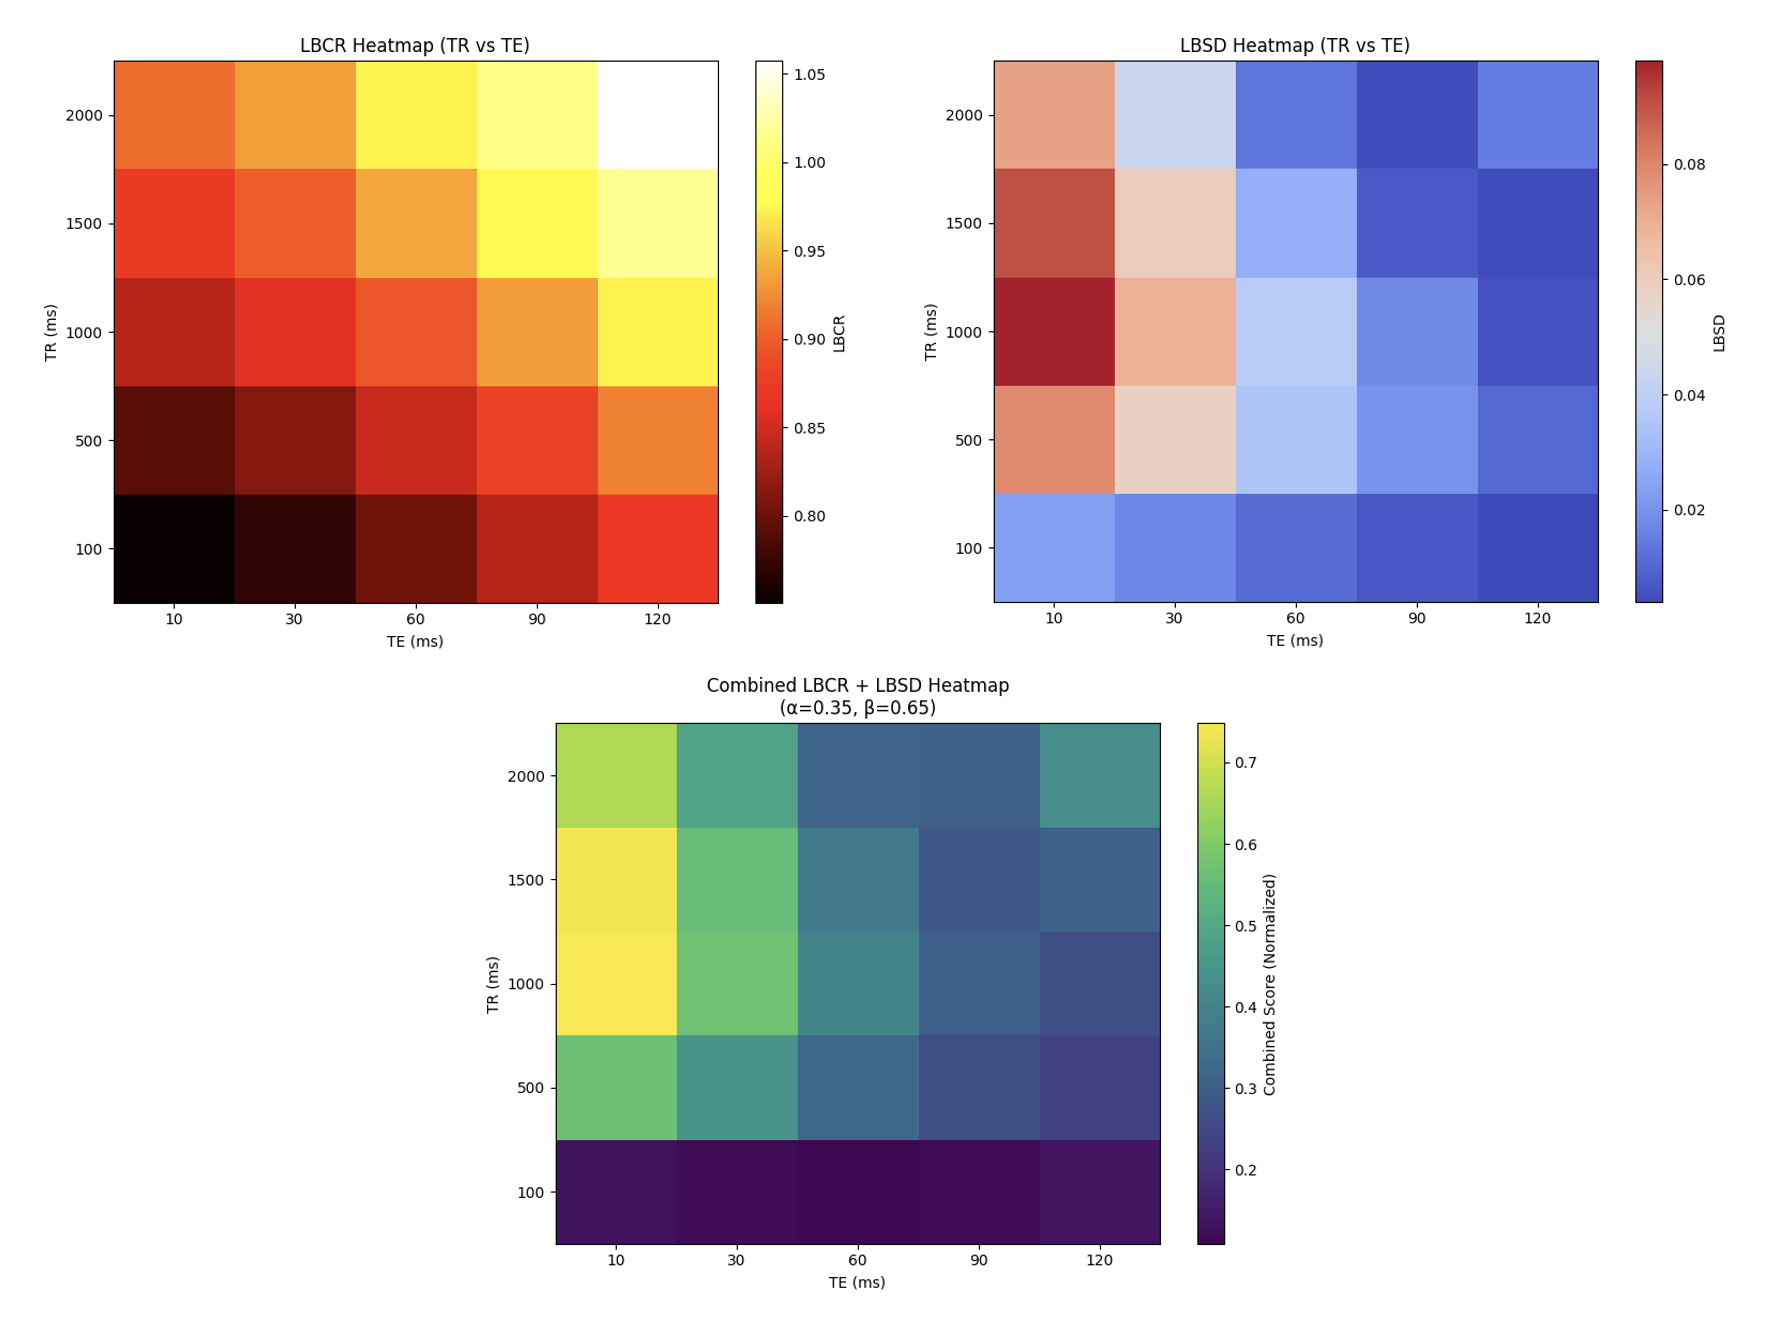
\includegraphics[width=\textwidth]{figures/lbcrlbsdcombinedheatmaps.png}
\caption{Top: Heatmaps of LBCR and LBSD variation over \( T_R \)-\( T_E \) space; Bottom: Combined LBCR-LBSD heatmap over \( T_R \)-\( T_E \) space, highlighting the optimal parameters at \( T_R = 1000 \) ms and \( T_E = 10 \) ms.}
\label{fig:lbcrsurface}
\end{figure}

Analysis of the combined LBCR-LBSD heatmap identified the optimal parameters at $T_R = 1000$ ms and $T_E = 10$ ms, where the combined metric maximized both lesion visibility and signal separation. This aligns with conventional $T_1$-weighted spin-echo imaging, where intermediate repetition times and short echo times enhance differences in longitudinal relaxation between tissues \cite{skalski2013}. This configuration is particularly effective for lesions exhibiting a radially decreasing gradient in both $T_1$ and $T_2$ values, as is often observed in high-grade gliomas. In such tumors, the periphery typically presents with vasogenic edema or infiltrative tumor tissue characterized by elevated $T_1$ and $T_2$, while the necrotic or hemorrhagic core exhibits shortened relaxation times due to increased cellularity, protein content, or hemosiderin deposition \cite{englund1986,blystad2017}. Consequently, a $T_1$-weighted acquisition emphasizes this relaxation gradient, producing dark cores and relatively bright peripheries—improving lesion visibility and internal heterogeneity.

To refine this result, bilinear interpolation over a finer 25×25 grid of $T_R$ and $T_E$ values revealed a slightly higher peak at $T_R = 1050$ ms and $T_E = 10$ ms, as shown in Figure~\ref{fig:lbcrlbsbinterpolated}. This sub-grid optimum validates the original discrete results as a close approximation while demonstrating how interpolation captures subtle enhancements missed at coarse resolution.

\begin{figure}[htbp!]
\centering
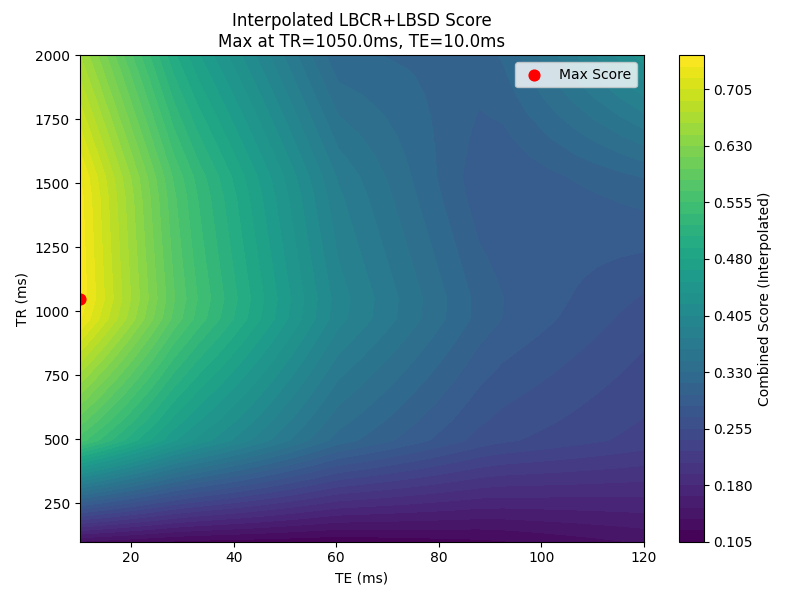
\includegraphics[width=0.75\textwidth]{figures/lbcrlbsdinterpolatedheatmap.png}
\caption{Interpolated LBCR-LBSD surface revealing a refined contrast maximum at $T_R = 1050$ ms and $T_E = 10$ ms, highlighting sub-grid contrast optimization.}
\label{fig:lbcrlbsbinterpolated}
\end{figure}

The arising prominence of intra-lesion heterogeneity we now see underscores its impact on contrast optimization. The radial gradients in $T_1$ and $T_2$ within the lesion, modeled to reflect pathological tissues like tumors, introduced complex signal variations that standard homogeneous models overlook \cite{does2002, xu2009}. For instance, the brighter lesion edge in $T_2$-weighted images, such as that in Figure~\ref{fig:inversion} ($T_R = 2000$ ms, $T_E = 100$ ms), resulted from its longer $T_2$, while the darker core reflected shorter $T_2$, aligning with experimental observations of lesion heterogeneity \cite{tofts2003}. Conversely, the optimal $T_R = 1000$ ms, $T_E = 10$ ms combination balanced $T_1$ and $T_2$ contributions, maximizing LBSD by preserving signal intensity across the lesion’s gradient.

While $T_2$-weighted imaging is valuable for delineating edema and tumor extent, especially in low-grade or infiltrative gliomas where transverse relaxation differences dominate, the use of a short $T_E$ in this simulation suppressed those transverse relaxation effects and favored contrast based on longitudinal recovery. In low-grade gliomas, where edema dominates the lesion microenvironment, $T_2$-weighted contrast is more informative. In contrast, necrotic cores in high-grade gliomas produce sharp $T_1$ gradients. 

To explore scenarios where $T_2$-weighting may be more advantageous, relaxation conditions may be simulated with parameters $T_1^{\text{bg}}, T_2^{\text{bg}} = 850, 80$ ms and $T_1^{\text{core}}, T_1^{\text{edge}} = 1200, 1400$ ms with $T_2^{\text{core}}, T_2^{\text{edge}} = 180, 250$ ms, which reflect more infiltrative or edematous tissue with elevated transverse relaxation. Under these conditions, longer $T_R$ and $T_E$ combinations may instead highlight peritumoral hyperintensities and diffuse infiltration better captured in $T_2$-weighted regimes. This supports the utility of $T_1$-weighted protocols for high-grade tumors with necrotic cores, while $T_2$-weighting may be preferential in low-grade or non-necrotic gliomas. Such differential contrast optimization may enhance downstream radiomic or diagnostic assessments targeting lesion heterogeneity across glioma subtypes.

These findings have significant implications for clinical MRI. The variability in LBCR and LBSD across $T_R$–$T_E$ space highlights the need for tailored acquisition parameters to enhance lesion detection, particularly in heterogeneous tissues. The combined LBCR-LBSD metric offers a quantitative approach to protocol optimization, reducing reliance on empirical testing and supporting reproducibility, as emphasized in recent quantitative MRI studies \cite{stikov2015, naganawa2002}.

This approach enables simulation-driven parameter tuning for specific tissue characteristics, potentially improving diagnostic yield and standardizing acquisition protocols for variable patient anatomies.


\section{Conclusion}

This study investigated how spatially varying relaxation parameters affect signal intensity and contrast formation in spin-echo MRI. By integrating voxel-wise $T_1$ and $T_2$ distributions into a 2D phantom and applying Bloch equation-derived signal modeling, the framework revealed how even subtle intra-lesional heterogeneity can produce pronounced contrast variations across the image. The results demonstrated the feasibility of mimicking realistic tissue textures through radial gradients and spatial smoothing, affirming the theoretical sensitivity of MRI signal contrast to both $T_1$ and $T_2$ variation and validating the decision to model relaxation behavior at the voxel level rather than assuming tissue uniformity.

The simulations, incorporating voxel-wise relaxation maps, reveal that contrast is highly sensitive to both acquisition parameters and intra-lesion heterogeneity. A key finding was the optimal LBCR at $T_R = 2000$ ms and $T_E = 120$ ms, which confirms the efficacy of $T_2$-weighted imaging for highlighting transverse relaxation differences. Meanwhile, a particularly insightful contribution of this study was the implementation of the LBSD, which is a quantifiable metric for evaluating image clarity. The simulations revealed a peak in LBSD at intermediate $T_R$ low $T_E$, revealing a nonlinear trade-off between signal intensity and contrast ratio that may inform optimized protocol selection. Taken together, these findings underscore the importance of tailoring acquisition settings to the underlying tissue relaxation dynamics and may guide improved imaging of biological substructures in clinical and radiomic workflows.

A combined metric for LBCR and LBSD, weighted at 0.35 and 0.65 respectively, further suggested a practical regime for balancing contrast and signal strength, with an interpolated global optimum found at $T_R = 1050$ ms and $T_E = 10$ ms. This approach extends prior work on signal modeling under relaxation variability by introducing a combined metric tailored to lesion imaging. The results also highlight the limitations of homogeneous tissue models, as the radial gradients in the lesion significantly altered signal patterns, consistent with experimental studies on tissue heterogeneity.

In summary, this project demonstrates that MRI signal simulations using spatially resolved relaxation maps are not only accurate representations of tissue contrast but also useful tools for protocol optimization. The LBCR-LBSD-based analysis adds a novel dimension to contrast evaluation, moving beyond qualitative assessments toward data-driven optimization. As clinical MRI moves toward quantitative and reproducible imaging, these findings offer a tractable strategy for protocol optimization. The computational simulation approach, grounded in the Bloch equations, enables rapid exploration of the parameter space without the constraints of experimental setups. 

This simulation framework has potential applications in preclinical research, teaching, and even aiding diagnostic imaging protocols by offering predictive insights on contrast behavior prior to empirical scanning. Future work could extend this framework to multi-compartment models or dynamic contrast-enhanced MRI, further bridging the gap between simulation and clinical practice.


\section{Recommendation}
To build on the outcomes of this simulation study, several recommendations are proposed for future work. First, the simulation framework can be extended to model more anatomically realistic tissue structures by incorporating non-radial lesion shapes or layered geometries that mimic gray and white matter. Introducing additional parameters such as proton density and diffusion properties could enhance the simulation’s ability to replicate a broader range of MRI sequences, including FLAIR and diffusion-weighted imaging. 

Furthermore, validating the LBCR-LBSD combined metric using real clinical datasets is encouraged, as it may serve as a quantitative benchmark for lesion visibility in diagnostic imaging. Expanding the model to three dimensions would also provide a richer platform for volumetric analysis, accounting for partial volume effects and slice thickness considerations. From an educational standpoint, this simulation could be developed into an interactive tool to help students and radiology trainees understand the effects of sequence parameters on contrast formation. 

Lastly, future studies may explore the use of machine learning algorithms to automatically predict optimal $T_R$ and $T_E$ settings for specific tissue types, potentially aiding in personalized MRI protocol design. These directions aim to enhance the realism, applicability, and pedagogical value of simulation-based MRI research.





% Please use the style file spp-bst.bst. If you wish to use BibTeX, kindly use us the filename bibfile.bib for your bib file.
\bibliographystyle{spp-bst}
\bibliography{bibfile}

\end{document}
